\begin{abstract}
In this user guide, I will introduce how to use this image inpainting software\footnote{This software is written by Hu Hu, Yesheng Ma, and Yikai Zou} both with the exemplar-based mode and the Markov random field mode. And I will illustrate my ideas using abundant figures.
\end{abstract}
\newpage


\section{Introduction}
First, we should give a definition of image inpainting and this is a first solid step to the success of our image inpainting software.

Most of you will have some old damaged photos at your home with some black or gray spots on it. It is really a real-world requirement to fix that image in an acceptable way. We can't simply erase them in a single color because it will simply replace the damaged region which is useless. In these cases, a technique called image inpainting is used. Look at the image bellow:
\begin{figure}[H]
\centering
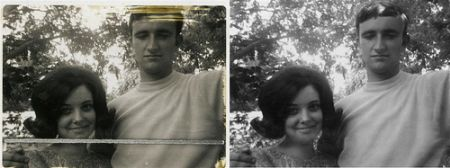
\includegraphics[width=9cm]{def.jpg}
\caption{An example of image inpainting}
\end{figure}
We can see that the left picture is damaged and
we want to fix those damaged regions. The right-hand-side picture is the in painted image, which is what we desire to get.
\newpage



\section{Architecture Requirements \& Installation}

\subsection{Computation platforms}
The recommended computation platform is shown as follows:
\begin{table}[H]
\centering
\begin{tabular}{|c|c|}
\hline
Hardware & Requirement \\ \hline
CPU & Intel Core i5 2GHz \\ \hline
Memory & 1GB \\ \hline
Disk & 100MB \\ \hline
GPU & N.A. \\ \hline
\end{tabular}
\caption{Hardware requirement spec}
\end{table}
Since to train the MRF model is CPU bound, we need the CPU to be at least Intel Core i5, which has a typical 2 GHz frequency. Also, our model is not typically designed for GPU and thus there is no limitation to GPU. For memory, the computation of MRF model requires much matrix computation and thus a 1GB memory is required. At last, we need to store the Berkeley image inpainting database, which contains 300 inpainted images and 100MB disk storage is required.
\subsection{Runtime environment requirement}
We want our image inpainting software to work cross-platform, thus a Windows OS or Linux OS will make sense.

As regard to programming language environment, we need a minimal MATLAB 2014 version in order to run our code in Windows OS. We recommend you use Python 2.7 instead of Python 3 since the libraries we use might not work fine with Python 3. Also, if you are using Linux, please make sure you have installed some cross-platform libraries such is python-tkinter so that our code can work
properly.
\subsection{Installation}
After you have installed all the above the dependencies, you can directly execute this image inpainting software. Following the README file in the root directory and enjoy this software.




\newpage

\section{Manual of exemplar-based algorithm}
\subsection{Input target image}
As is shown in the following figures, when we click the left button, we can select the input image from the file system of current user and after we selected the input image, the selected image will be immediately shown on the window, which provides perfect user interaction experience.

\begin{figure}[H]
\centering
\begin{subfigure}{0.45\textwidth}
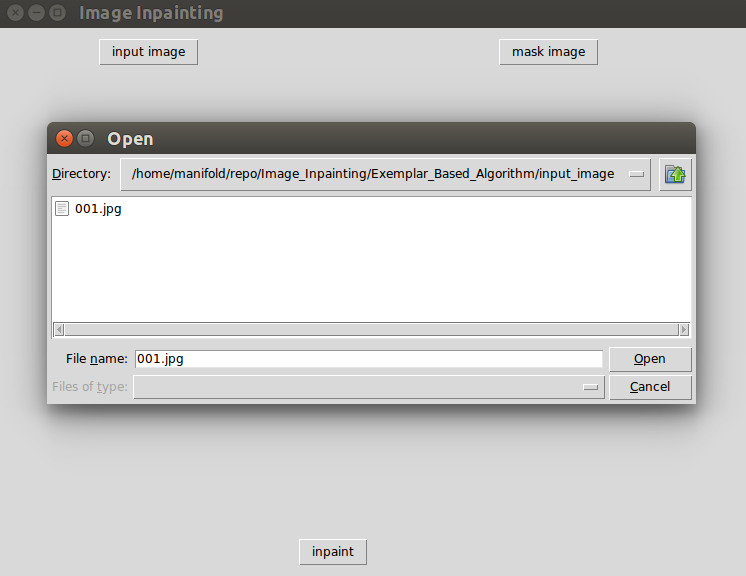
\includegraphics[width=\textwidth]{ex_input.png}
\caption{Select input image}
\end{subfigure}
~
\begin{subfigure}{0.45\textwidth}
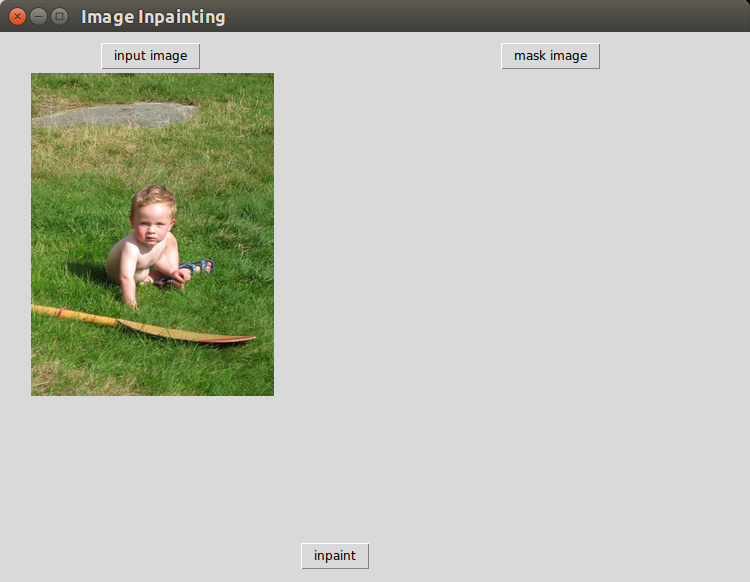
\includegraphics[width=\textwidth]{ex_input_img.png}
\caption{Display input image}
\end{subfigure}
\caption{Input image use case}
\end{figure}

\subsection{Input mask image}
use not only need to provide an input image, but also an input mask so that the computer can get aware of which part should e inpainted. As well as the case of input image, we can select the desired mask from user file system and the mask will be shown on the screen as soon as the user chooses proper input mask.

\begin{figure}[H]
\centering
\begin{subfigure}{0.45\textwidth}
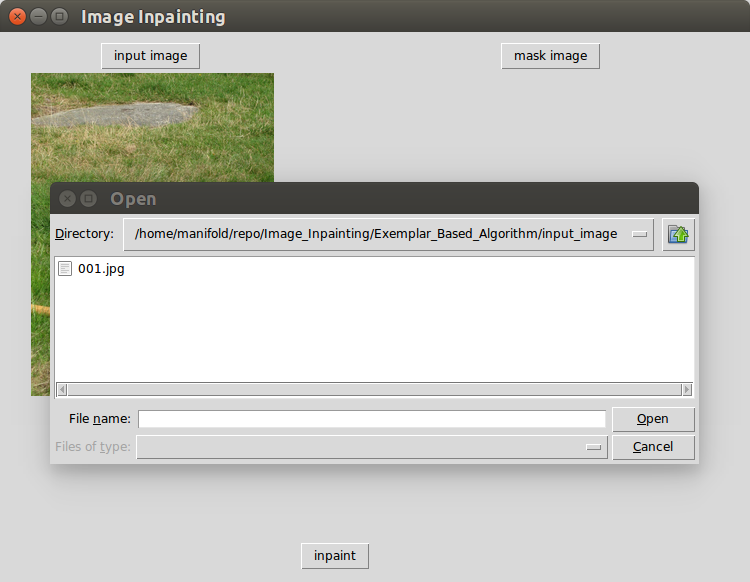
\includegraphics[width=\textwidth]{ex_mask.png}
\caption{Select input mask}
\end{subfigure}
~
\begin{subfigure}{0.45\textwidth}
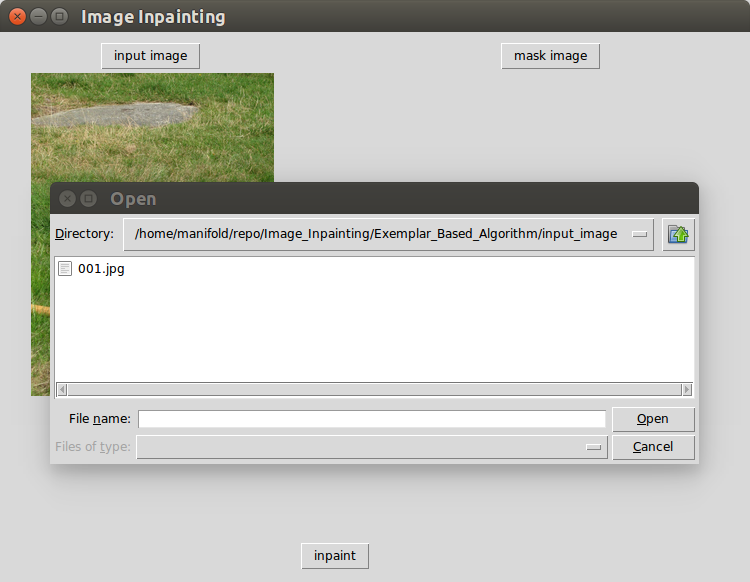
\includegraphics[width=\textwidth]{ex_mask.png}
\caption{Display input mask}
\end{subfigure}
\caption{Input mask use case}
\end{figure}

\subsection{Execution of inpainting}
Once we have inputed both the target image and input mask, we can click the ``inpaint'' button to start execution. During the execution of the inpainting program, the image inpainting software will regularly save the partially inpainted image to disk and we can further look at that image to checkout how much have been inpainted.
\begin{figure}[H]
\centering
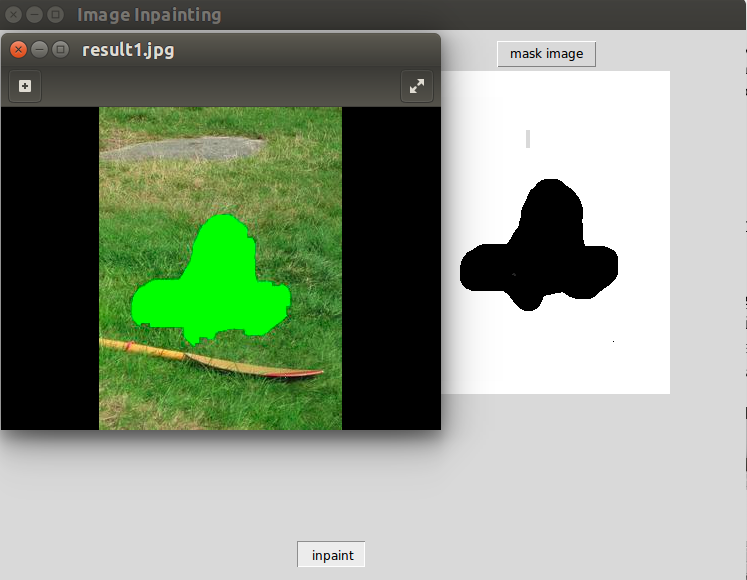
\includegraphics[width=9cm]{ex_ex.png}
\caption{Image inpainting process}
\end{figure}
From the above image we can clearly see that some part of the image has already been inpainted
\subsection{Checkout result image}
Once the inpainting process finishes, we can checkout the result. The following figure show the result of inpainting.
\begin{figure}[H]
\centering
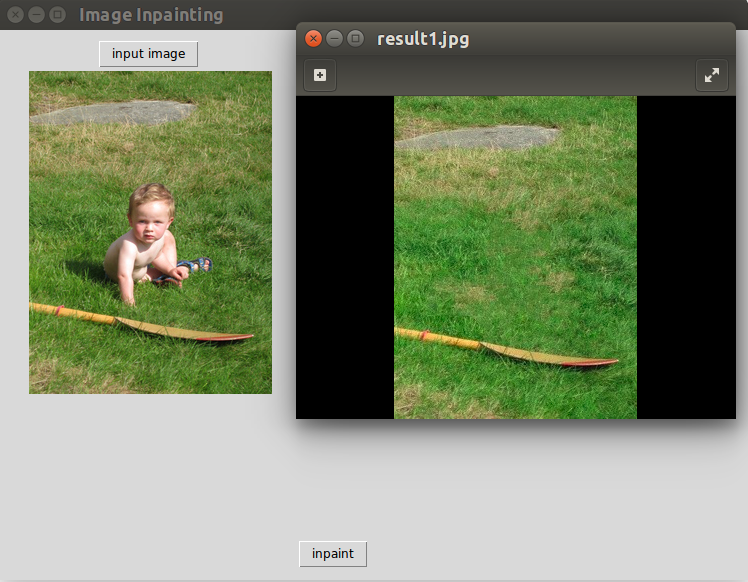
\includegraphics[width=9cm]{ex_res.png}
\caption{Image inpainting result}
\end{figure}
As we can see from this figure, the result of inpainted image is quite good.

\newpage
\section{Manual of Markov random field}
In this section, we will discuss the use case of another completely different algorithm: Markov random field. Since it is convenient to read in a file in MATLAB, we will no longer discuss file IO in detail with respect to MRF method. We will mainly talk about the convergence here.
\subsection{Monitor status}
Once we hit the start key, the Markov random field model will begin to compute on this image. The computation will continue until the model converges.

However, the user may not be aware of how much the model has been fitted. So we provide a window to display the extent of convergence and we will update this window to keep it up-to-date.

At beginning, the trend of convergence might not seem obvious. As is shown in the following figure, there are three lines in the figure, which has colors of red, green, and blue, and you might cleverly discover that represents the convergence three different convergence trend of RGB(red, green, blue) channels.

\begin{figure}[H]
\centering
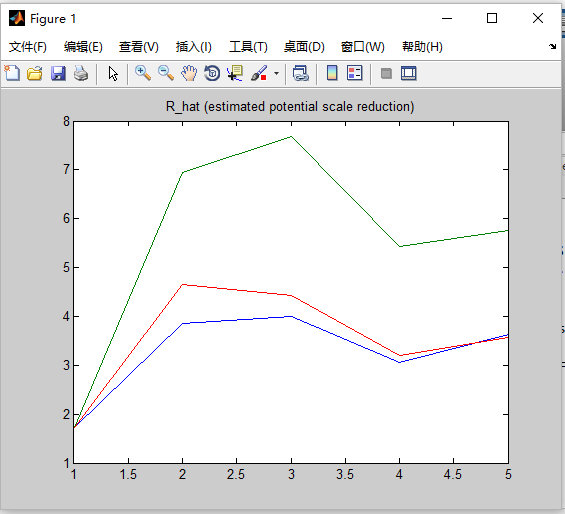
\includegraphics[width=8cm]{mrf_beg.png}
\caption{Beginning of convergence}
\end{figure}

As the process of computation continues, we will see that the value $\hat{R}$ will drop dramatically since this value represents the estimated potential scale reduction, where the potential is a terminology in Markov random field representing the probabilistic distribution over a small region of pixels.

\begin{figure}[H]
\centering
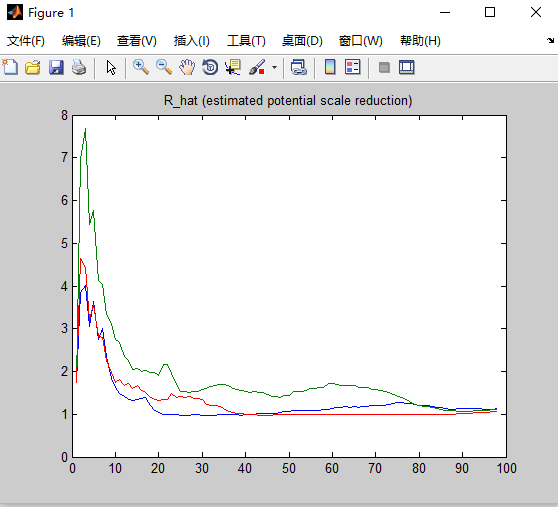
\includegraphics[width=8cm]{mrf_cov.png}
\caption{Near the end of convergence}
\end{figure}

As we can see from the above figure, both the RGB channels are near the end of convergence (when we say end of convergence, we mean that the scale reduction of RGB both become 0).

\subsection{Result demonstration}
After the final convergence, a window of both the original figure and the inpainted figure will show on the screen. The following figure shows the result of inpainted image, which is a inpainted image of one of our teammates:

\begin{figure}[H]
\centering
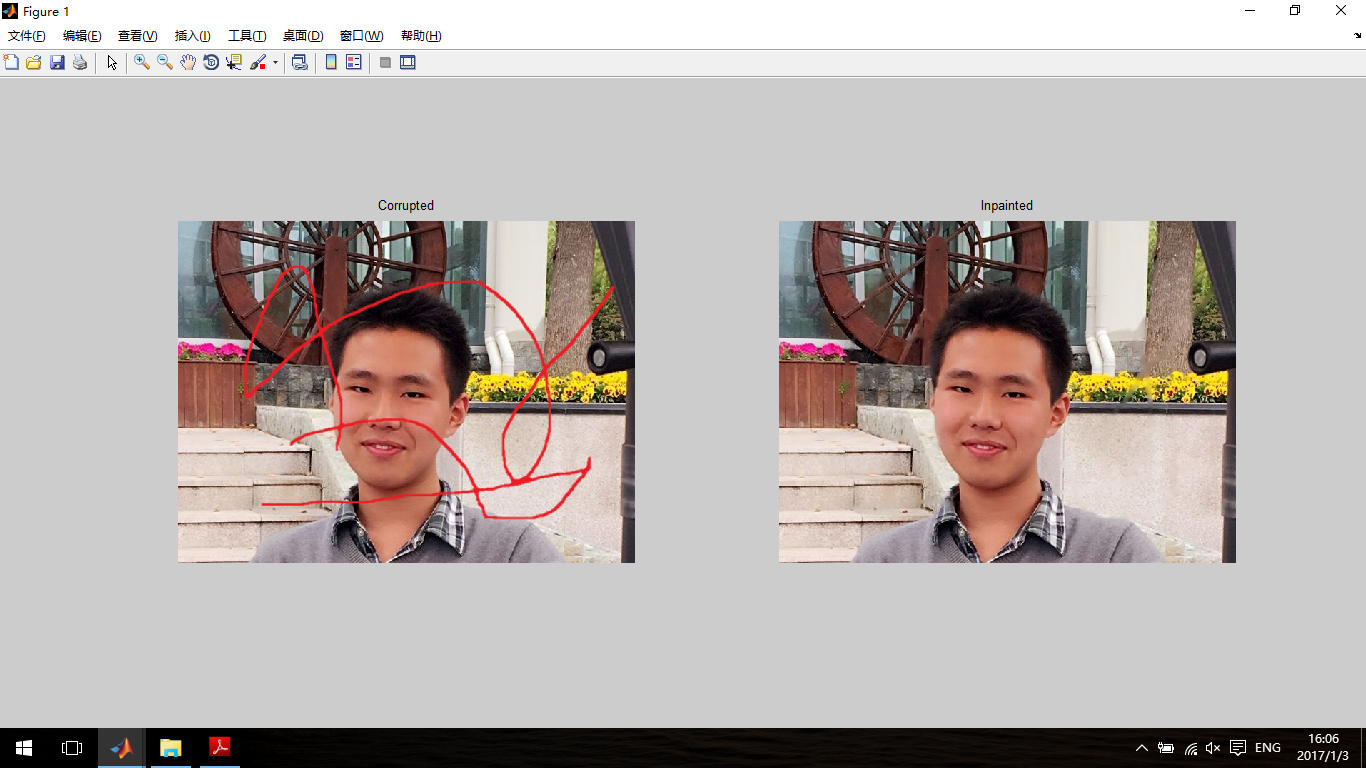
\includegraphics[width=8cm]{mrf_res.png}
\caption{Result of Markov random field model}
\end{figure}

As we can see from the above figure, we have a damaged image on the left, after the model has converged, we have the fixed image on the right and the fixed image restores the fixed image quite well.


\newpage
\section{Other Use Cases}
Apart from fix image and object removal, there are many other use cases of image inpainting. Here we will give another use case to inspire the reader to come up with more interesting use cases. This example use case remove the unwanted text from a given image. The input image is as follows:
\begin{figure}[H]
\centering
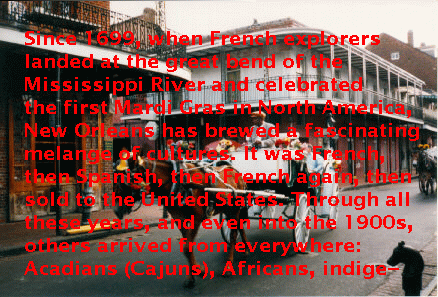
\includegraphics[width=6cm]{hc.png}
\caption{Image with unwanted text on it}
\end{figure}
We can apply either the exemplar-based algorithm or Markov random field on it. Here we apply the Markov random field algorithm on it since it work best on such small region restoration. The following figure shows the fixed version:
\begin{figure}[H]
\centering
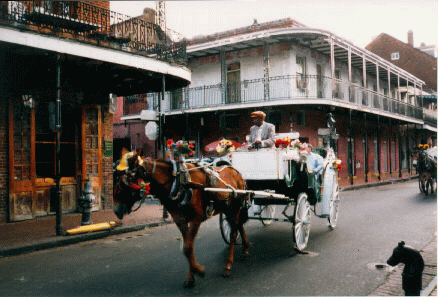
\includegraphics[width=6cm]{hc_res.png}
\caption{Image with unwanted text removed}
\end{figure}
Although making musk for this image might be a little tedious, it would be much more tedious if one uses software like PS to fix such an image.


\newpage
\section{Conclusion}
That's all for this user guide. Since the principles used in this image inpainting software is really complicated and we might not convey it well in such a short user guide. If you have any problem or you want to report bugs, you can go to \texttt{https://github.com/MihawkHu/Image\_Inpainting} for help and we are looking forward for your feedback.